\chapter{Vorbereitung}

\section{Der klassische Hall-Effekt}

Der klassische Hall-Effekt beschreibt den Effekt eines Magnetfeldes auf eine
Probe. So baut sich im Inneren der Probe ein elektrisches Feld auf, dessen
resultierende elektrische Kraft im stationären Zustand gerade die Lorentz-Kraft
kompensiert.\\
Zur Diskussion beginnt man mit der klassischen Bewegungsgleichung im Magnetfeld:
\[
    m^* \dot{\vec{v}} = - e \left( \vec{E} + \vec{v}_d \times \vec{B} \right)
                      - m^* \frac{\vec{v}_d}{\tau}
\]
Hierbei bezeichnet $\vec{v}_d$ die Driftgeschwindigkeit, $\tau$ die mittlere
Stoßzeit, $m^*$ die effektive Masse, $\vec{E}$ das elektrische Feld und $\vec{B}$
das Magnetfeld. Der Term $-e \vec{E}$ beschreibt die durch das elektrische 
Gleichfeld auf die Elektronen wirkende konstante Kraft. Der letzte Teil 
$m \, \vec{v_d} / \tau$ berücksichtigt die hemmende Wirkung der Stöße. 
Da die Elektronen bei jedem Stoß ihre Bewegungsrichtung ändern, bleibt außerdem
nur der durch die Driftgeschwindigkeit verursachte Beitrag 
$-e \left( \vec{v}_d \times \vec{B} \right)$ übrig.\\
Zur Vereinfachung betrachten wir ein in $z$-Richtung anliegendes Magnetfeld
im stationären Fall, also $\dot{\vec{v}} = 0$. Somit ergibt sich:
\begin{align*}
    \vec{v}_{d,x} &= - \frac{e \tau}{m^*} \left( E_x + \vec{v}_{d,y} \; B \right),\\
    \vec{v}_{d,y} &= - \frac{e \tau}{m^*} \left( E_y + \vec{v}_{d,x} \; B \right),\\
    \vec{v}_{d,x} &= - \frac{e \tau}{m^*} E_z
\end{align*}
Mit der Beweglichkeit $\mu = e \tau / m$ und der Elektronendichte
\[
    j = -e n \vec{v}_d = \frac{n e^2 \tau}{m} \vec{E} = n e \mu E
\]
aus der für die elektrische Leitfähigkeit folgt
\[
    \sigma = \frac{j}{E} = \frac{n e^2 \tau}{m} = n e \mu
\]
folgt für die Stromdichte im betrachteten Fall:
\[
    \begin{pmatrix}
        j_x\\ j_y \\ j_z
    \end{pmatrix} 
    = - \frac{\sigma_0}{1 + \omega_c^2 \tau^2}
      \begin{pmatrix}
          1             & -\omega_c \tau    & 0 \\
          \omega_c \tau & 1                 & 0 \\
          0             & 0                 & 1+\omega_c^2 \tau^2 \\
      \end{pmatrix}
      \begin{pmatrix}
          E_x \\ E_y \\ E_z
      \end{pmatrix}
\]
Hier bezeichnet $\omega_0 = n e^2 \tau / m^*$ die Leitfähigkeit ohne Magnetfeld
und $\omega_c$ für die Zyklotronfrequenz.\\
Zur Vereinfachung betrachten wir einen flachen Stab mit rechteckigen Querschnitt.
Der Strom fließt hierbei in $x$-Richtung. Mit dieser Geometrie tritt in
$z$-Richtung kein elektrisches Feld auf. Somit vereinfacht sich obiger Ausdruck zu:
\[
    \begin{pmatrix}
        j_x \\ j_y
    \end{pmatrix}
    = \begin{pmatrix}
         \omega_{xx} & \omega_{xy} \\
        -\omega_{xy} & \omega_{xx}
      \end{pmatrix}
      \begin{pmatrix}
          E_x \\ E_y
      \end{pmatrix}
\]
Hier wurden die Leitwerte
\[
    \omega_{xx} = \frac{ne}{B} \frac{\omega_c \tau}{1+\omega_c^2 \tau^2}, \qquad
    \omega_{xy} = -\frac{ne}{B} \frac{\omega_c^2 \tau^2}{1+\omega_c^2 \tau^2}
\]
eingeführt.\\
Löst man das Gleichungssystem nach den elektrischen Feldern auf erhält man:
\[
    \begin{pmatrix} E_x \\ E_y \end{pmatrix}
    = \begin{pmatrix}
         \rho_{xx} & \rho_{xy} \\
        -\rho_{xy} & \rho_{xx} 
      \end{pmatrix}
      \begin{pmatrix}
          j_x \\ j_y
      \end{pmatrix}
\]
mit den spezifischen Widerständen:
\[
    \rho_{xx} = \frac{B}{ne} \frac{1}{\omega_c \tau} = \frac{m^*}{ne^2\tau}, \qquad
    \rho_{xy} = \frac{B}{ne}
\]
Hier wird $\rho_{xx}$ als Längswiderstand $R$ und $\rho_{xy}$ als Hall-Widerstand
$R_H$ bezeichnet.
In einem anisotropen Medium würden die Größen $\rho_{yx}$ und $\rho_{yy}$
auftreten. Für isotrope Medien, die hier betrachtet werden sollen, gilt jedoch:
$\rho_{xx} = \rho_{yy}$ und $\rho_{yx} = - \rho_{xy}$. Ein Plot der klassischen
Widerstände ist in Abbildung \ref{Abb:klassisch} zu sehen.
\begin{figure}
    \centering
        \begin{subfigure}[c]{0.45\textwidth}
        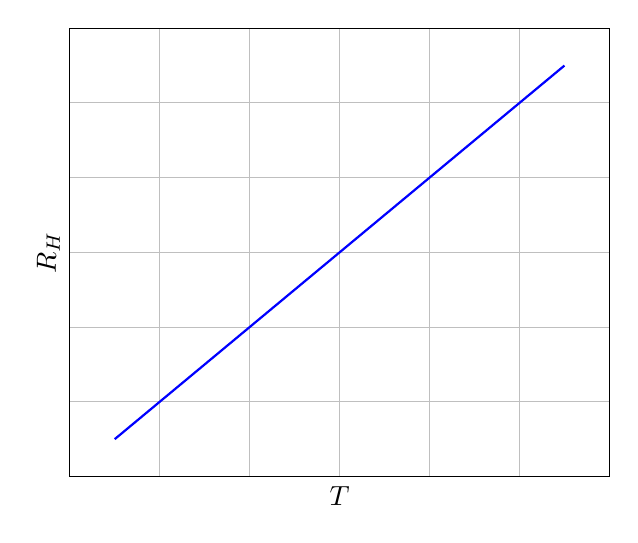
\begin{tikzpicture}
            \begin{axis}[
                ticks=none,
                xlabel={$T$}, ylabel={$R_H$},
                grid=both
            ]
                \addplot[thick, blue] {x};
            \end{axis}
        \end{tikzpicture}
        \caption{Hall-Widerstand}
    \end{subfigure}
    \begin{subfigure}[c]{0.45\textwidth}
        \begin{tikzpicture}
            \begin{axis}[
                ticks=none,
                xlabel={$T$}, ylabel={$R_\square$},
                grid=both
            ]
                \addplot[thick, blue] {1};
            \end{axis}
        \end{tikzpicture}
        \caption{Schichtwiderstand}
    \end{subfigure}

    \caption{Widerstände beim klassischen Hall-Effekt}
    \label{Abb:klassisch}
\end{figure}

\section{Quanten-Hall-Effekt}
\subsection{Zweidimensionales Elektronengas}

Die Untersuchung des Quanten-Hall-Effekts wird an einem sog. Zweidimensionales 
Elektronengas durchgeführt. Hierbei handelt es sich um ein freies Elektronengas, 
also die Elektronen können sich näherungsweise frei in alle Raumrichtungen bewegen,
dass in einer Raumrichtung durch einen schmalen Potentialtopf eingeschränkt wird.
Dies führt zu einer Quantisierung der Gesamtenergien, die ein Elektron haben kann.
Ist nun nur das unterste Niveau besetzt, so können sich die Teilchen in zwei 
Richtungen frei bewegen, während sie in die dritte eingesperrt sind. Somit ergibt
sich der Begriff des Zweidimensionales Elektronengases.\\\\
Zur theoretischen Betrachtung wählt man den Potentialtopf zur Vereinfachung in 
$z$-Richtung. Die Energie in z-Richtung ist somit quantisiert und darstellbar als
$E_{s} (s=0,1,\dots)$. Für die Gesamtenergie eines Elektrons ergibt sich:
\[
	E(s,k_{x},k_{y}) = E_{s} + \frac{\hbar^{2} k_{x}^{2}}{2m^{*}}
					   + \frac{\hbar^{2} k_{y}^{2}}{2m^{*}}, \qquad{}
	(s=0,1,\dots)
\]
$E_{s}$ ist unabhängig vom Wellenvektor $\vec{k}$, da in $z$-Richtung keine 
Bewegung stattfindet. Die beiden hinteren Terme beschreiben die kontinuierliche
freie Bewegung in der $x-y$-Ebene. $m^{*}$ bezeichnet die effektive Masse.

\subsection{Theorie des Quanten-Hall-Effekt}

Misst man den Hall-Effekt nun an einem Zweidimensionalen Elektronengas bei wenigen
Kelvin und Magnetfeldern im einstelligen Teslabereich, so weicht das Ergebnis vom
klassischen Hall-Effekt ab. Ein Beispiel dafür ist in Abbildung \ref{Abb:qhe} 
dargestellt.

\begin{figure}[ht]
    \centering
    \def\svgwidth{0.6\linewidth}
    \import{Abb/}{quanten_hall.pdf_tex}
    \caption{Hall und Schichtwiderstand beim Quanten-Hall-Effekt}
    \label{Abb:qhe}
\end{figure}

Bei kleinem Magnetfeld deckt sich der Graph mit dem linearen Anstieg beim
klassischen Hall-Effekt. Bei größeren Feldern bilden sich Plateaus bei bestimmten 
Widerstandswerten aus:
\[
	R_{H} = \frac{1}{\nu} \frac{\hbar}{e^{2}}, \qquad (\nu=1,2,\dots)
\]
Dies wird als Quanten-Hall-Effekt bezeichnet.
Gleichzeitig oszilliert der Längswiderstand bei hohen Feldstärken. Die wirkliche
ist jedoch sehr viel kleiner als der Hall-Widerstand. In Abbildung \ref{Abb:qhe}
wurden deshalb beide Werte normalisiert, um die Lesbarkeit zu verbessern. 
Die Minima der Oszillationen, bei denen der Längswiderstand verschwindet, liegt auf
den Plateaus des Hall-Widerstands. Dieses Phänomen wird als
Shubnikov-de-Haas-Oszillation bezeichnet.\\\\
Zur theoretischen Betrachtung stellt man folgende Schrödingergleichung auf:
\[
	\left(
		\frac{( i\hbar\nabla+e \, \vec{A}(x,y) )^{2}}{2m^{*}} + U(y)
	\right) \Psi(x,y) = E \, \Psi(x,y)
\]
Hier wählt man $\vec{A} = (-By,0,0)$, sodass $\vec{B} = rot \vec{A}$ in $z$-Richtung
zeigt. Das Randpotential $U(y)$ schränkt die Elektronenbewegung auf die Ausdehnung
der Probe ein.
Weiter wird nun eine eine ausreichend große Probe angenommen, sodass $U(y)$ 
vernachlässigt werden kann:
\newcommand{\zweim}{\frac{1}{2m^{*}}}
\[{}
	\zweim \left( (p_{x} + e B y)^{2} + p_{y}^{2}\right) \Psi(x,y) = E \Psi(x,y)
\]
$p_{x} = - i \hbar \partial_{x}$ und $p_{y} = - i \hbar \partial_{y}$ bezeichnen die
Impulsoperatoren in $x$- bzw. $y$-Richtung.
Zur Lösung wird nun der Separationsansatz verwendet:
\[
	\Psi(x,y) = \phi(x) \chi(y) = \frac{1}{\sqrt{L}} \exp(ikx) \chi(y)
\]
Für $\chi(y)$ muss also gelten:
\[
	\zweim \left[ (\hbar k + eBy)^{2} + p_{y}^{2} \right] \chi(y) = E \chi(y)
\]
Diese Gleichung kann in die Schrödingergleichung eines eindimensionalen,
harmonischen Oszillators umgeformt werden. Hierzu wird die Frequenz
$\omega_{c} = \frac{e B}{m^{*}}$ und die Zentrumskoordinate 
$y_{k} = \frac{\hbar k}{eB}$ eingeführt. Durch einfaches Einsetzen ergibt sich:
\[
	\left[ \frac{p_{y}^{2}}{2m^{*}} + \frac{1}{2} m^{*} \omega_{c}^{2}
	(y + y_{k})^{2} \right] \chi(y) = E \chi(y)
\]
Die Frequenz des harmonischen Oszillators ist die eingeführte Frequenz $\omega_{c}$.
Die Koordinate $y_{k}$ bezeichnet die Verschiebung des harmonischen Oszillators auf
der $y$-Achse vom Nullpunkt.
